\chapter{Design} \label{cha:design}
\section{Technology Choices} \label{sec:chapdesign:technology}
This section will discuss choices that have been made throughout the project regarding technology used and justifications for their usage.

\subsection{Rust} \label{sec:chapdesign:technology:rust}
There were a few requirements when choosing an appropriate programming language for this project:
\begin{enumerate} 
    \item Performance: Optimization is crucial for IoT devices due to their limited processing power. Server performance can be scaled more easily, however is still an important consideration.
    \item Stability: The language should encourage memory-safe and error-handled code, as IoT devices and their servers need to run for long periods without crashes and memory leaks.
    \item Security: The language should promote secure coding practices. A blog-post by the "Microsoft Security Response Centre" states that 70\% of all vulnerabilities assigned a CVE (Common Vulnerabilities and Exposures) each year are due to memory corruption errors \cite{ProactiveApproachToSecureCode}.
    \item Ease of Use and Comfort: A user-friendly language can speed up development and design iteration, possibly improving the final product, but familiarity with a language can compensate for this.

\end{enumerate}
The language that was chosen for this project was Rust. While C/C++'s performance rivals and often surpasses Rust, the difference is often quite marginal \cite{PerformanceEvalOnMicrocontroller}, due to all three being compiled to machine code. What makes Rust different, is its headline feature, known as the "borrow checker". It can ensure that at compile-time, the code is memory safe. Due to the code being guaranteed memory safe at compile time, outside explicitly marked unsafe blocks, Rust code is known for its ability to run long-term without running into crashes. Additionally, Rust code is a popular choice for embedded devices, due to being able to compile without a standard library, giving it flexibility in a project such as this. Finally, even though it is known as a difficult language to learn and master, personal familiarity with Rust makes it an obvious choice for this project.

\subsection{gRPC} \label{sec:chapdesign:technology:grpc}
gRPC is an RPC implementation released by Google in 2015. It uses Protocol Buffers (protobufs) as an interface definition language (IDL), to define services on servers, that clients can then call. The server runs a gRPC server and the client runs the gRPC client \cite{grpcHomepage}. Protobufs can be compiled to many different languages, including Rust and Typescript. In a performance comparison between REST, gRPC, websockets and GraphQL, gRPC came out ahead in many different metrics \cite{reviewOfInternetProtocols} in both native and containerized tests. In fact, gRPC was the most performant internet communication protocol in all metrics apart from memory usage.

Due to its performance and cross-language support I have chosen gRPC as the internet communication protocol for this project. The specific library used for this project is known as "Tonic". Tonic is a Rust gRPC crate that includes both a gRPC server and client. It also utilizes an additional Rust library named "prost", to compile protobuf files into Rust code, without having to interface the protobuf compiler itself. 

\subsection{Typescript \& VueJS} \label{sec:chapdesign:technology:ts}
While a Command Line Interface (CLI) frontend, written in Rust, will be made available, the main focus will be on the Graphical User Interface (GUI). To ensure that it can run on a variety of systems and is relatively easy to create, it will be web based, using Javascript at runtime. However, it will be written in Typescript. Typescript is a superset of Javascript, that compiles to Javascript and leaves no trace of types behind. Typescript provides a robust type-system, including, but not limited to \cite{understandingTypescript}:
\begin{itemize}
    \item Structural type equivalence, instead of Javascript's by-name type equivalence
    \item Types and concepts for object-based programming
    \item Type operators
\end{itemize}
All of these, while not guaranteeing that the program will be type-safe at runtime, help a developer design more robust and long term solutions generally associated with statically typed languages.

In conjunction with Typescript a web-development framework will be used. Web frameworks are libraries for Javascript that allow easier development of websites and web apps, often incorporating HTML (HyperText Markup Language) and CSS (Cascading Style Sheets) code into Javascript code. They also provide reactivity, meaning that if a variable changes in the code, that change can easily be reflected on the site. This can be done in most frameworks by simply using the variable in the HTML code, something that standard HTML does not support (methods of doing this differs between frameworks).

Web-framework choice often hinges on personal preference and familiarity. Performance differences exist between frameworks, but they’re usually negligible and shouldn’t dictate choice. While there is a lack of formal experiments on framework performance, an informal experiment \cite{performanceComparisonJS} shows performance differences between most major frameworks being negligible. Due to this and personal familiarity with the framework, VueJS was chosen for this project’s frontend. 


\section{System Architecture} \label{sec:chapdesign:architecture}

The overall system architecture can be seen in figure~\ref{fig:system_architecture}.
\begin{figure}[h]
\caption{System Architecture}
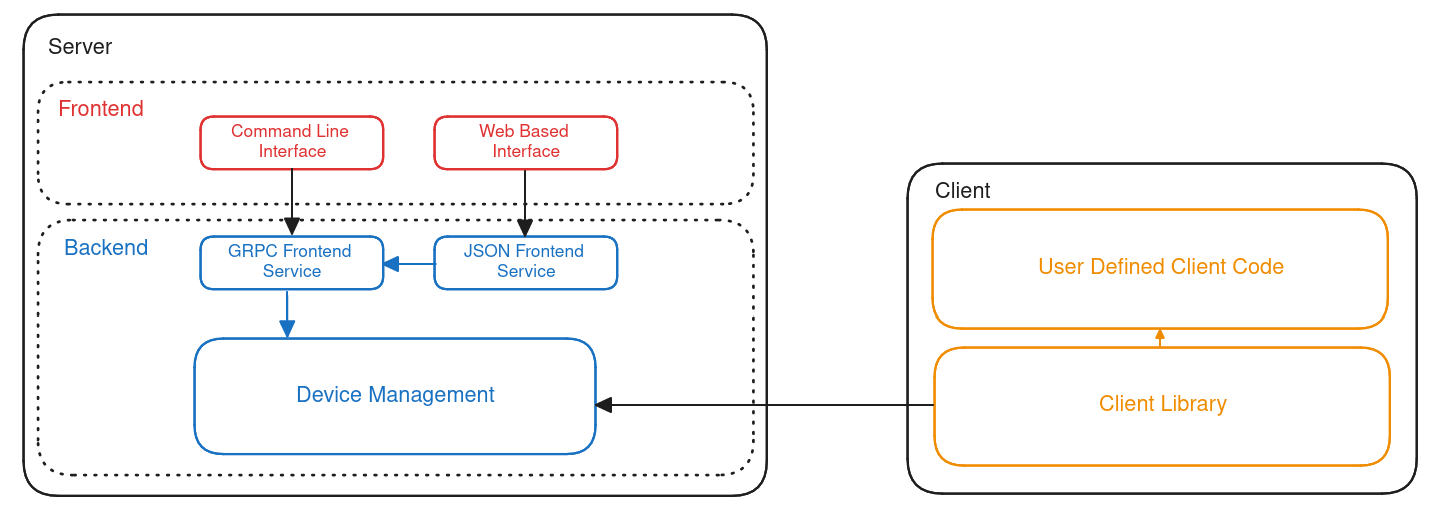
\includegraphics[width=\textwidth]{system_architecture.png}
\label{fig:system_architecture}
\end{figure}
This system architecture consists of two main components, the server and the client. Here the server represents the main controller of the system. The client is any device connected to the system (there most likely will be multiple). One peculiarity, is the fact that the frontend is contained by the server part of the system. This is because, in the current design, by default the frontend will be run on the same machine as the backend, with frontend API endpoints (located in the frontend services) being open on the localhost loop back address. This can however be easily changed by a user, by simply changing the address the frontend API endpoints are hosted on.

The arrows in the architectural diagram represent the direction of contact. For example, a client can contact the backend and the backend may respond, however the backend cannot contact a device, it can only reply to a request. The only deviation from this rule is within the client. At startup, the user will supply the client library with callback functions, which the library can call. This means that the user defined code must be able to contact the client library during setup. However, once the client library has finished setup and has created contact with the backend, the user defined code can no longer interact directly with the client library. The library will then simply call any code supplied to it during setup, without having any direct contact with user defined code.

Figure~\ref{fig:device_management_architecture} shows the architecture of the "Device Management" part of the backend of the system architecture.
\begin{figure}[h]
\caption{Device Management Architecture}
\centering
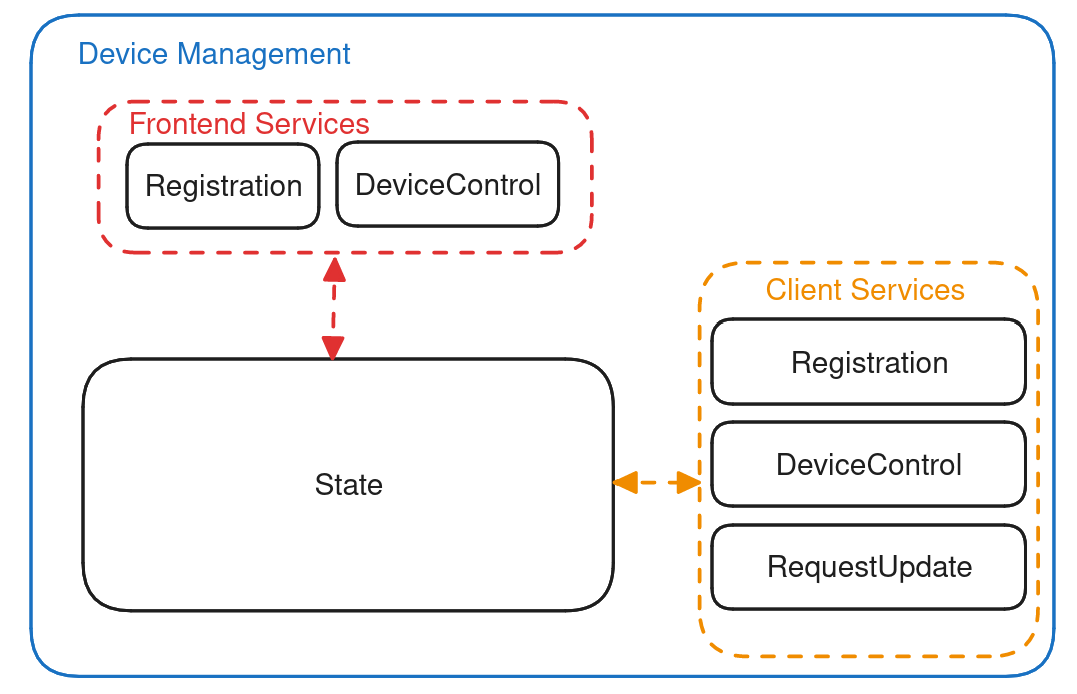
\includegraphics[width=0.7\textwidth, height=0.30\textheight]{device_management_architecture.png}
\label{fig:device_management_architecture}
\end{figure}
Device Management is comprised of several services, being based on the SBA architecture discussed in section~\ref{sec:chap2:architectures}. Each service has its own function and is independent. However, they all access the same state and are all defined in protobuf files and can therefore all having functions that can be called using gRPC.


\section{Security} \label{sec:chapdesign:security}
As previously discussed, security is an important concern within a smart-home environment. The user of the system is putting trust into the system to behave as it is meant to, while keeping their personal data safe from outside intruders. That is why special care will be put into the security aspects of the system. This will come in a two pronged approach using certificates and signatures. 
\subsection{Certificates}
A certificate is a tool for verifying that a client is who they say they are. It is generated by the server and can be verified by the server. This is useful, for example, if the client goes offline and at a later time wants to re-aunthenticate with the server. They can send the certificate provided to them earlier and the server can verify it. The certificate scheme that will be implemented is based on \cite{disSysConceptsDesign}.

Figure~\ref{fig:certificate_exchange} shows the certificate exchange protocol that will be used, where cK is the client key pair and sK is the server key pair. K(pub) represents the public key part of the key pair.
\begin{figure}[h]
\caption{Certificate Exchange}
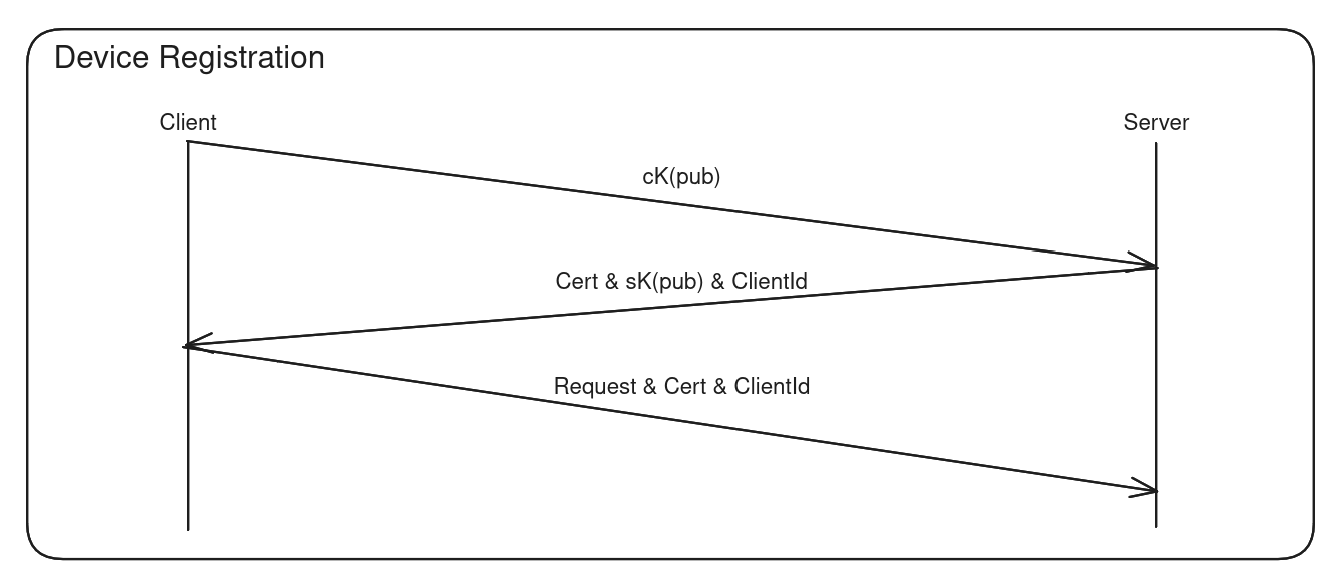
\includegraphics[width=\textwidth]{certificate_exchange.png}
\label{fig:certificate_exchange}
\end{figure}

At startup the server and client will both generate an asymmetric key pair using the Rivest, Shamir, Adleman (RSA) public key system. Then, during registration, the client will send the server their public key. The server then creates csr where \(csr = cK(pub) + ClientId\). Csr is then hashed using SHA256 hashing to create the certificate: \(certificate = H_x(csr)\). This certificate is then sent back to the client, along with the server public key and their client identifier (which is a UUID randomly generated by the server). Now, if the client goes offline and wants to re-register, instead of having to repeat the registration process again, they can simply include their certificate instead and be verified by the server. Verification is quite simple. The client simply re-generates csr using the client's public key and client-id, then re-hashes them. If the new hash is the same as the certificate, then the client is verified.

\subsection{Signatures}
Signatures allow both the server and client to verify that the messages they are receiving are not forged and sent by a third party. The signatures will use the key-pairs generated and exchanged during registration (view certificate exchange), to sign every message with a hash, that can be independently verified by the other party. The message sender will use their private key to sign their message and the receiver will use the public key send during registration to verify the message. This signature scheme is based on concepts described within \cite{disSysConceptsDesign} and \cite{disSysPrinciples}.

Every signature will consist of three important parts:
\begin{enumerate}
    \item Unix Timestamp - This will be used to prevent replay attacks. Every message will include the Unix timestamp of when it was sent and this information will be included in the signature. The receiver can then check the age of the message and discard it if it is beyond a certain threshold.
    \item Message Contents - This is used to ensure that the contents of the message stay the same between sender and receiver. Because hashing the entire contents of a message might be costly, some subset of the contents must be chosen. This will depend on the message type.
    \item Certificate - The certificate is included in the hash, however not in the message. This is an extra layer of security, as both server and client have an independent version of the certificate, meaning that an attacker would also need to obtain this certificate somehow, along with the private key of the sender.
\end{enumerate}

Every message will include a signature, which must first be verified by the receiver before the information within the message is processed. This is help ensure that data can not be tampered with between sender and receiver.


\section{Web Frontend} \label{sec:chapdesign:frontend}
Figure~\ref{fig:home_screen_mockup} shows a mockup what the home-screen of the web frontend should look like. The main focus should be on the devices, which will be represented by boxes on the home screen. The device's available capabilities will be shown as buttons or sliders, configurable from the device itself. As the focus of this project is mainly on the system and the API of the device server will be available, custom web frontends should be easy to make, for a more customizable experience. Due to the whole project being open-source, this frontend can be built upon by other users, or companies, interested in customizing it.

\begin{figure}[h]
\caption{Home Screen Mockup}
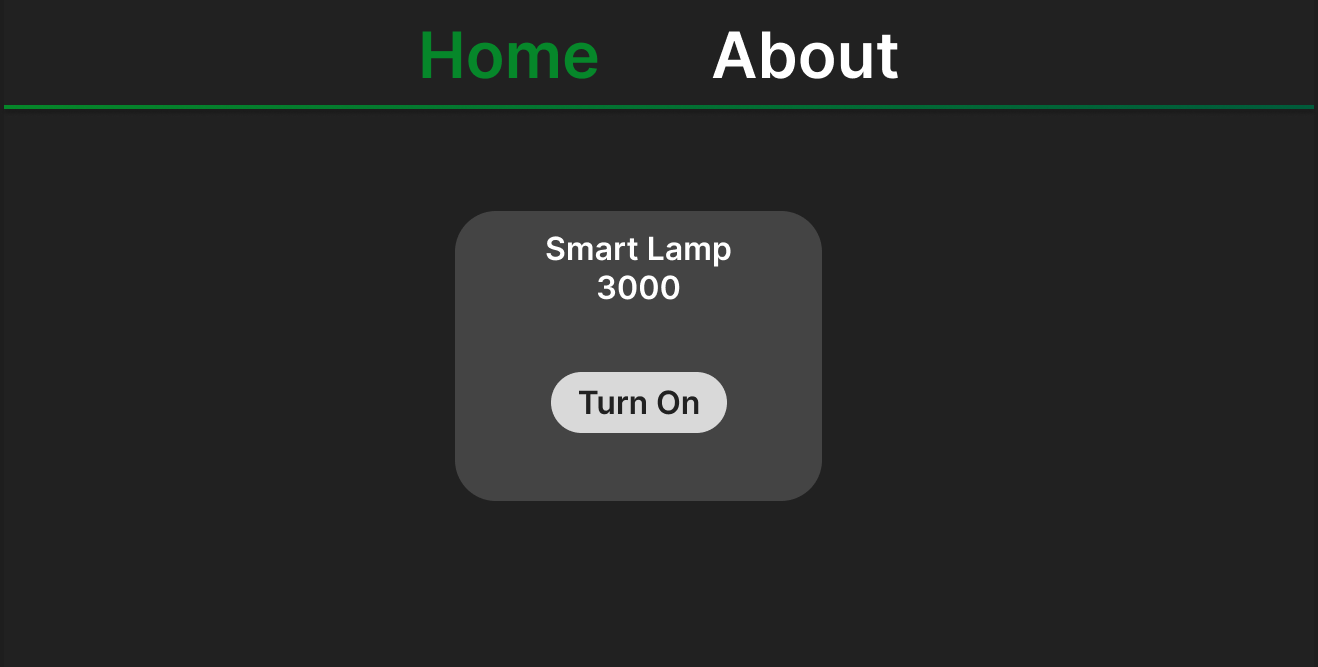
\includegraphics[width=\textwidth]{homescreen_design.png}
\label{fig:home_screen_mockup}
\end{figure}

